%
% latex-sample.tex
%
% This LaTeX source file provides a template for a typical research paper.
%

%
% Use the standard article template.
%
\documentclass{article}

% The geometry package allows for easy page formatting.
\usepackage{geometry}
\geometry{letterpaper}

% Load up special logo commands.
\usepackage{doc}

% Package for formatting URLs.
\usepackage{url}

% Packages and definitions for graphics files.
\usepackage{graphicx}
\usepackage{epstopdf}
\DeclareGraphicsRule{.tif}{png}{.png}{`convert #1 `dirname #1`/`basename #1 .tif`.png}

%
% Set the title, author, and date.
%
\title{Dating Website Interfaces}
\author{Joseph Crawley}
\date{September 18, 2012}

%
% The document proper.
%
\begin{document}

% Add the title section.
\maketitle

% Add an abstract.
\abstract{}
For this assignment, Terran Moore and I looked how Match.com, Eharmony.com, and ChristianMingle.com measured in the usability metrics of Learnability, Satisfaction, and Efficiency. For this assignment, we had 5 users create profiles and complete similar tasks in order to measure these metrics.  

% Add various lists on new pages.
\pagebreak
\tableofcontents


%\listoffigures


%\listoftables

% Start the paper on a new page.
\pagebreak

%
% Body text.
%
\section{Learnability}
\label{Learnability}

\subsection{E-harmony.com}
Users were able to fill out profiles almost instantly. Searching was hard to understand and users became frustrated with the searching of the system.

\subsection{Match.com}
Menus were easy to understand and users could fill out profiles almost instantly. The searching function was easy to pick up on for users, and users could navigate the site with ease.

\subsection{ChristianMingle.com}
The site was very simple and easy to understand. Menus were clearly marked, and everything was labeled very quickly.


\section{Efficiency}
\subsection{E-harmony.com}
E-harmony was efficient on every test except for search ability, which it tested very poorly in. Its search ability was foreign to users who were familiar with networking sites and caused users to be frustrated.

\subsection{Match.com}
Match.com was very intuitive to users for all aspects. Users felt that they could navigate the site quickly and efficiently with little errors and with a low learning curve.

\subsection{ChristianMingle.com}
Users liked how simple ChristianMingle.com was. They felt that the simplicity helped them navigate the site easily. The only thing that was not simple was updating profile information, which took users a few more clicks than necessary.


\section{Satisfaction}
\subsection{E-harmony.com}
Users felt this site was very good for something, but bad for dating itself. Users felt that it was next to impossible and very timely to connect with matches. Users had low satisfaction with the site.


\subsection{Match.com}
	Users felt that this was the preferred choice in dating websites. It combined the comprehensiveness of E-harmony with the comprehensiveness of Match.com. Users were happy with how quick they picked up the site and how natural the interface was.

\subsection{ChristianMingle.com}
Users felt Christian Mingle was easy to use, but too simple. Users did not feel that the creating a profile interface was comprehensive enough. Although the menus were simple, they felt that the actions they wanted to take were not always available in the menus.

\section{Expectations of Dating Interfaces}

For our report, we could not find any specific reference or guide specific to dating websites, so we used the government usability guidelines. The below sections will contain excerpts from usability.gov, and how they are seen on the dating websites.

\subsection{"Designers should make every attempt to reduce the user’s workload by taking advantage of the computer’s capabilities."}
Since dating websites often require a lot of input when making a profile, dating websites should have efficient ways to enter data and also vary in data entry style so that the user does not become bored.

\subsubsection{E-harmony.com}
When filling out a profile on E-harmony, the user is asked a serious of personality questions. Almost all of the questions were in the formal as seen in Figure \ref{Eharm1}. The users in our tests often felt that they were bombarded with questions. The E-harmony questionnaire was the longest, therefore took our users the longest to fill out. Our users were frustrated with the amount of questions, and since most of the questions were in the same format, our users were bored and began to answer questions quickly and less efficiently. E-harmony could change the style of how they ask questions after every few responses.

\begin{figure}
\centering
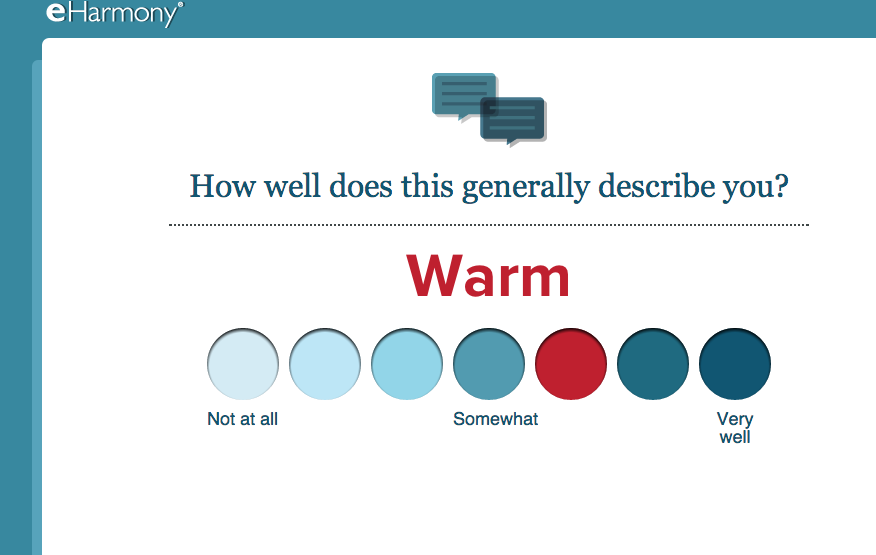
\includegraphics[width=4in]{Eharm1.png} 

\caption{E-Harmony personality questions}
\label{Eharm1}
\end{figure}

\subsubsection{Match.com}
Match.com does a good job of asking question multiple ways. Like Figure \ref{Match1}, there are 4-7 questions on a page, and there are multiple ways to submit input on this page. This kept users on their toes and stopped users from blindly answering questions. The only drawback to this interface is that the users spent more time per question than they did with E-Harmony. Users had to adjust answering in different ways, which made the questionnaire take more time.  

\begin{figure}
\centering
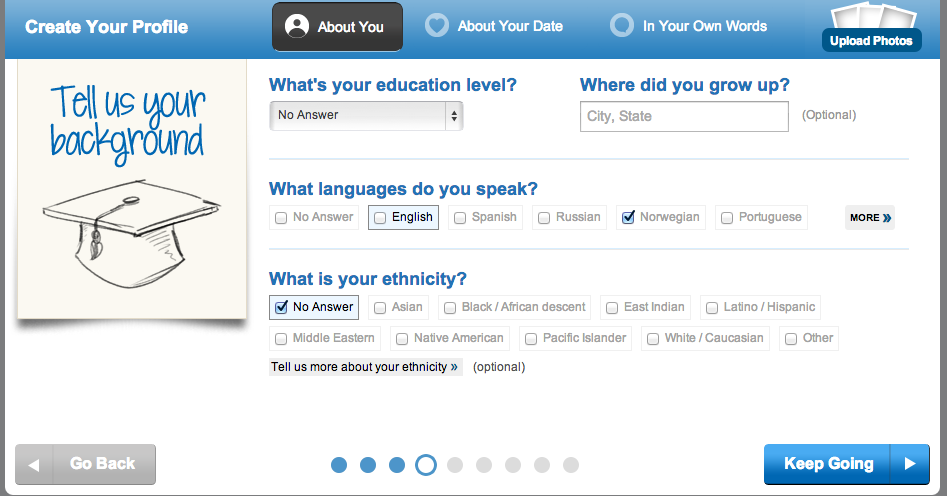
\includegraphics[width=4in]{Match1.png} 

\caption{Match.com personality questions}
\label{Match1}
\end{figure}

\subsubsection{ChristianMingle.com}
Just like E-Harmony, Christian Mingle only used one type of input submission for its questions. However, Christian Mingle had a lot fewer questions than E-Harmony, so the user never had the opportunity to be bored by reading questions. The only concern with the question form was that there was no way to change answers if mistakes were made. Besides that, questions were easy to answer and process.

\begin{figure}
\centering
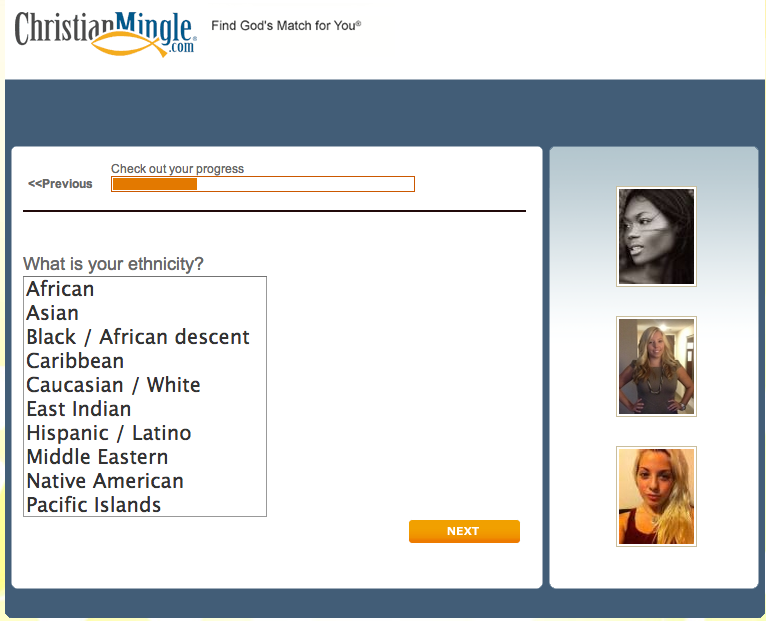
\includegraphics[width=4in]{CM1.png} 

\caption{ChristianMingle.com personality question page}
\label{CM1}
\end{figure}

\subsection{“Results of user searches provide the precise information being sought, and in a format that matches users’ expectations.”}



\pagebreak
% Generate the bibliography.
%\bibliography{intro}
%\bibliographystyle{plain}

\end{document}
